\section{Vårt Arbeid}

\subsection{Utstyrsliste} % Må da finnes en penere måte

Veroboard, 32 sockets

Kretskort gitt til lab i TFE4101

Digital Oscilloskop - Rohde \& Schwarz RTB2004

Signalgenerator - Rohde \& Schwarz HMF2525

Spenningskilde - Rohde \& Schwarz HMC 8042

Banankabler

BNC-BNC kabler

BNC-banankabel

BNC-splitter

Prober

\subsection{Forarbeid}

\subsubsection*{Design av absoluttverdikrets}

I forarbeidet skulle det designes en 4-bits absoluttverdikrets.
For å ta absoluttverdien av et binært tall kan man invertere det og addere 1.
En absoluttverdikrets kan dermed bygges opp av inverterkretser og av halvadderkretser.
Vi startet med å designe en inverterkrets, altså en krets som inverterer hvert bit som kommer inn, hvis kretsen er aktivert.

Det blir gjort tydelig av tabell \ref{tabell:1} at en slik krets kan lett implementeres som en XOR-port.

\begin{table}[h]
  \centering
  \begin{tabular}{c c|c}

    In & En & Out\\
    \hline
    0 & 0 & 1\\
    0 & 1 & 0\\
    1 & 0 & 1\\
    1 & 1 & 0\\

  \end{tabular}
  \caption{Sannhetstabell for inverterkrets}
  \label{tabell:1}
\end{table}

% \begin{figure}
%   \centering
%   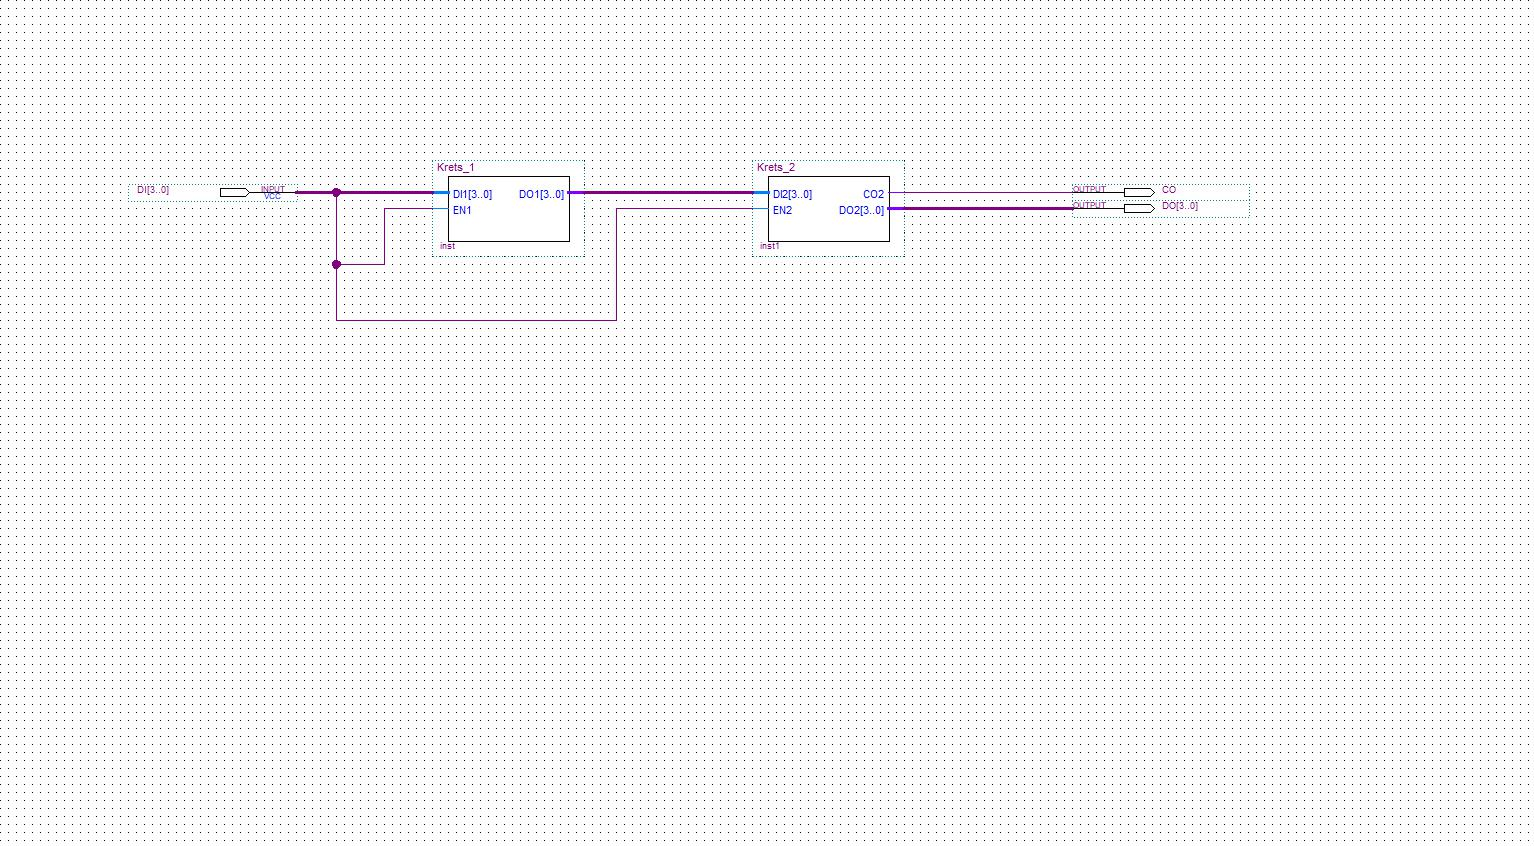
\includegraphics{4 bit abs}
%   \caption{}
%   \label{}
% \end{figure}

Deretter designet vi en halvadderkrets. En halvadderkrets adderer to tall og har to utganger, en for summen og en for mente, så lenge kretsen er aktivert.

\begin{table}[h]
  \centering
  \begin{tabular}{c c|c|c}

    In & Carry-In & Sum & Carry-Out\\
    \hline
    0 & 0 & 0 & 0\\
    0 & 1 & 1 & 0\\
    1 & 0 & 1 & 0\\
    1 & 1 & 0 & 1\\

  \end{tabular}
  \caption{Sannhetstabell for halvadderkrets}
  \label{tabell:2}
\end{table}

% \begin{figure}
%   \centering
%   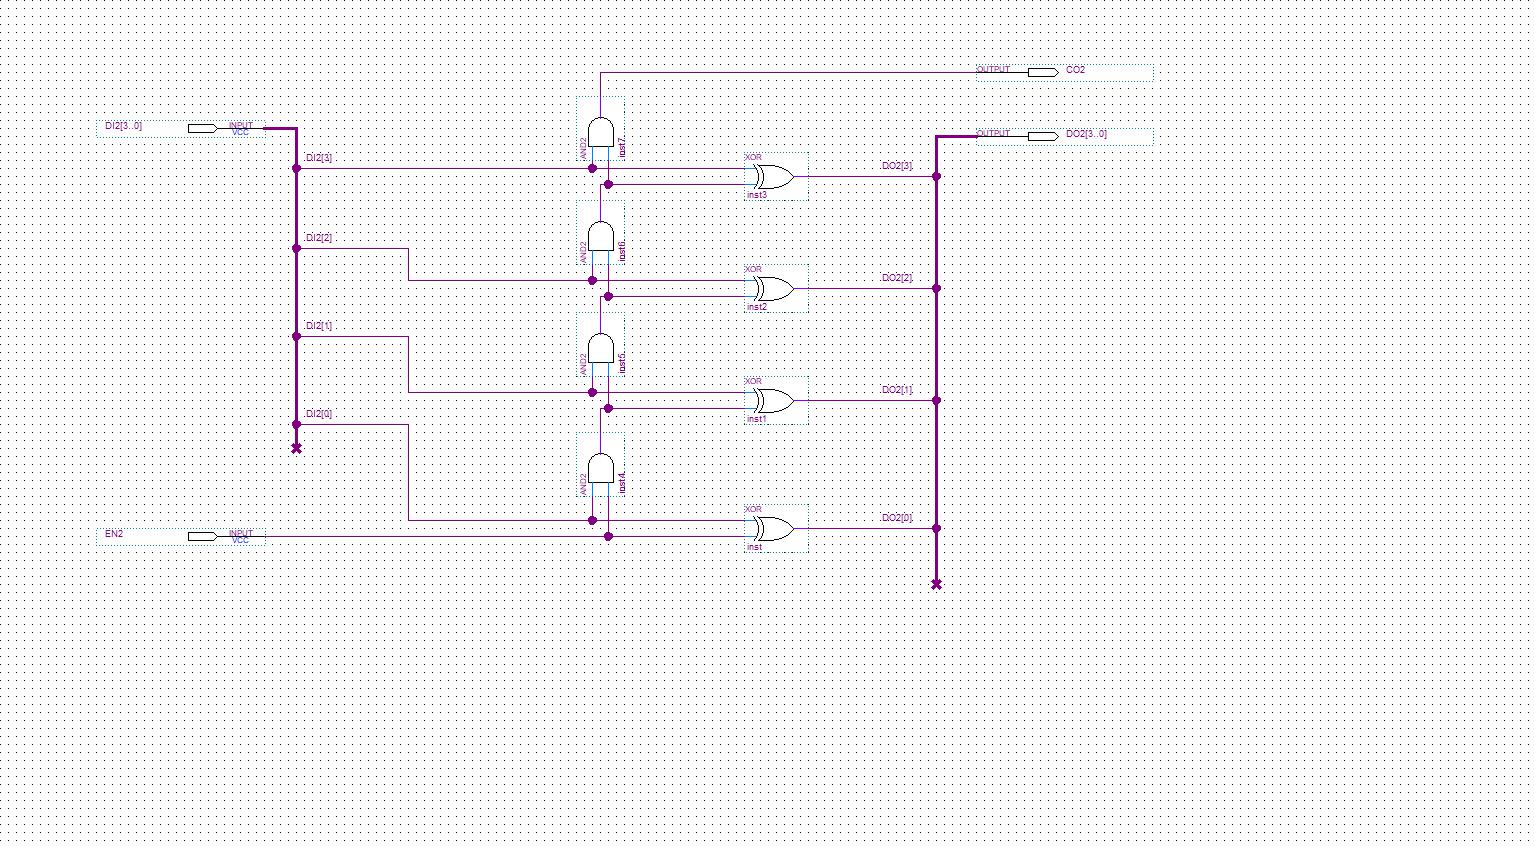
\includegraphics{4 bit adder}
%   \caption{}
%   \label{}
% \end{figure}

Etter å ha designet disse komponentene, måtte vi sette de sammen til å bli en 4-bits absoluttverdikrets.
Da lagde vi blokker ved å sette inverterkretsen og halvadderkretsen i serie, og satte fire av disse blokkene i parallell.
Videre brukte vi MSB som enable signal for inverterne og som mente inn for første halvadder, slik som i Figur

\begin{figure}[h]
  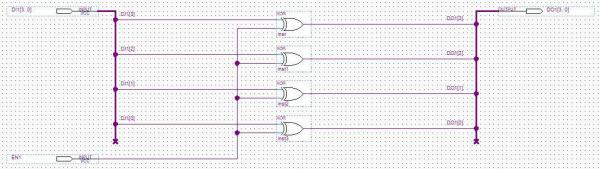
\includegraphics{4BitInverter.jpg}
  \caption{4-bits inverter}
  \label{figur:1}
\end{figure}

\subsubsection*{Beregning av kritisk sti og maksimal klokkehastighet}

Kritisk sti fant vi ved å se på det scenarioet hvor det blir flest menteforplantninger, nemlig overgangen fra 1000 til 1000, hvor det skjer menteforplantninger gjennom hele kretsen.
Da går kritisk sti gjennom 2 XOR porter og 3 AND porter.
For å beregne forsinkelsen gjennom kritisk sti fant vi verdiene for forsinkelse gjennom de forkjellige portene ved 5V som maks spenning, som er som gitt i Tabell \ref{tabell:3}

\begin{table}[h]
  \centering
  \begin{tabular}{c c}

    Port & Forsinkelse\\
    \hline
    AND & 125ns\\
    XOR & 140ns\\

  \end{tabular}
  \caption{Forsinkelsestid gjennom porter}
  \label{tabell:3}
\end{table}

Gitt disse verdiene kan vi regne oss frem til forsinkelse gjennom kritisk sti.

\begin{displaymath}
  2 \cdot 140ns + 3 \cdot 125ns = 655ns
\end{displaymath}

Dette gir oss at maksimal klokkehastighet er:

\begin{displaymath}
  \frac{1}{655ns} = \SI{1.53}{\mega\hertz}
\end{displaymath}

\subsection{Labarbeid}

\subsubsection*{Kobling av halvadderkrets}

Før vi startet på labarbeidet sørget vi for å resette alt av utstyr som kunne resettes.
Deretter kunne vi begynne med første del av labarbeidet, som var å koble opp en halvadderkrets på veroboardet.
Da satte vi kretskortet i sokkelen og koblet på 7DC fra spenningskilden inn til terminal 31 og jord til terminal 32.

Videre koblet vi halvadderkretsen som følger:
\begin{displaymath}
  28 \rightarrow 16, 14
\end{displaymath}
\begin{displaymath}
  27 \rightarrow 15, 13
\end{displaymath}

Etter at vi koblet opp kretsen testet vi den etter Tabell \ref{tabell:2}. Alle verdier stemte overrens.

\subsubsection*{Kobling av absoluttverdikrets}

Etter å ha koblet opp og testen halvadderkretsen koblet vi den ut og koblet til en absoluttverdikrets som vist i Figur \ref{Kretstegning:1}
Deretter testen vi kretsen etter Tabell \ref{Tabell:5}. Alle verdier stemte.

\subsubsection*{Forplantningsforsinkelse}

Før vi målte forsinkelsestid gjennom kretsen ble proben kalibrert etter instruksjoner på oscilloskopet.
Deretter koblet vi sammen spenningskilden, oscilloskopet og veroboardet slik som i Figur \ref{Kobling:1}.
På veroboardet ble positiv koblet til terminal 27 og jord i terminal 32.
Signalgeneratoren ble satt til å generere en firkantpuls mellom 0V og 5V med en frekvens på 100kHz.

Deretter koblet vi proben til kretsen med jord som 32 og proben til ben på chippen som vist i Figur \ref{figur:2}

\begin{figure}[h]
  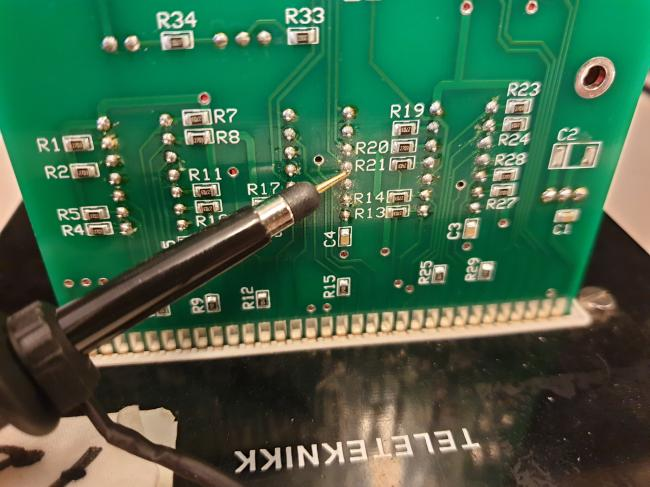
\includegraphics{Bilder/Probetest1}
  \caption{Test av forsinkelse gjennom kretsen}
  \label{figur:2}
\end{figure}

Forplantningsforsinkelsen ble målt til 543,2ns. Gitt dette har vi at avviket fra den beregnede verdien er:

\begin{displaymath}
  \cfrac{543,2ns}{655ns}\cdot100\%=17\%
\end{displaymath}

Det at vi fikk lavere forplantningstid enn forventet kan muligens skyldes varmeutvikling i komponentene, men vi har ingen garanti for dette.
Gitt den målte forplantningsforsinkelsen får vi en ny maksimal klokkehastighet.

\begin{displaymath}
  \cfrac{1}{543,2ns}=\SI{1,84}{\mega\hertz}
\end{displaymath}

Etter dette brukte vi oscilloskopet til å sjekke hva som skjer hvis man øker frekvensen på signalgeneratoren til og forbi 50\% av maksimal klokkehastighet.
Resultatene vi kom frem til var at hvis frekvensen når 50\% av maksimal klokkehastighet, så blir input lav idet output blir høy.
Mens hvis frekvensen går over 50\% av maksimal klokkehastighet blir forplantningsforsinkelsen større.

\subsubsection*{Rise Time og Fall Time}

Før vi begynte med nye målinger stilte vi signalgeneratoren tilbake til 100kHz.
For måling av stige- og falltid for en XOR-port ble proben værende i samme posisjon som for måling av forplantningsforsinkelsen, ettersom den siste porten i kritisk sti var en XOR-port.
Stige- og falltiden ble målt med de innebygde funksjonene "Rise Time" og "Fall Time" i oscilloskopet og sjekket ved hjelp av "cursorfunksjonen" grafisk, på skjermen til oscilloskopet.

For måling av stige- og falltid for en AND-port ble proben flyttet til posisjonen gitt i Figur \ref{figur:3}
Videre ble samme prosedyre som for XOR-porten brukt.

\begin{figure}[h]
  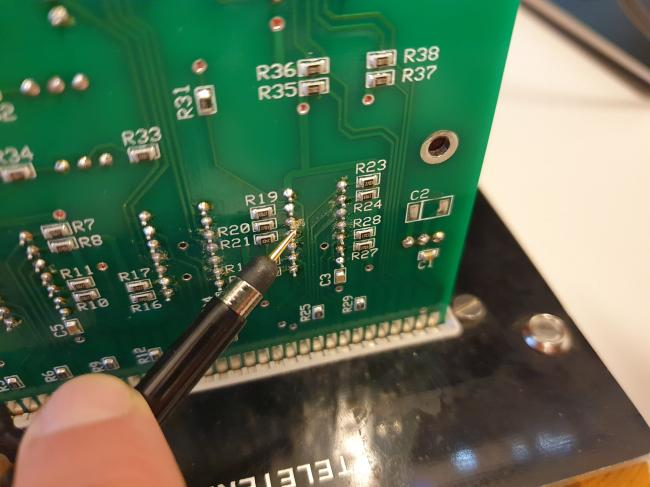
\includegraphics{Bilder/Probetest2}
  \caption{Test av Rise Time og Fall Time i AND-port}
  \label{figur:3}
\end{figure}

Resultatene av disse målingene finner du i Tabell \ref{stigetidstuff}
